\subsection{UC16 - Ricerca prodotto per nome}
\begin{figure}[H]
  \centering
  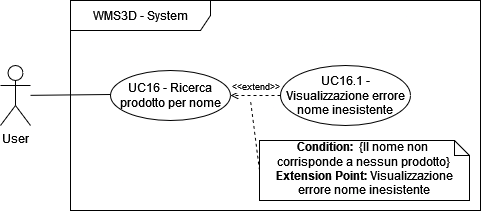
\includegraphics[width=0.8\textwidth]{UC_diagrams_11-20/UC16.drawio.png}
   \caption{Diagramma UML UC16}
\end{figure}
\begin{itemize}
    \item \textbf{Attori:} User.
    \item \textbf{Pre-condizione:} L'utente ha creato un magazzino [UC1].
    \item \textbf{Post-condizione:} L'utente può cercare un prodotto dando in input un nome e può visualizzarne i risultati [UC17].
    \item \textbf{Scenario Principale:} L'utente inserisce un nome per ricercare il prodotto corrispondente. I risultati della ricerca possono poi essere visualizzati [UC17].
    \item \textbf{Generalizzazioni:} -
    \item \textbf{Estensioni:} È presente una estensione:
    \begin{itemize}
        \item UC16.1 - Visualizzazione errore nome inesistente.
    \end{itemize}
\end{itemize}


\subsubsection{UC16.1 - Visualizzazione errore codice inesistente}
\begin{itemize}
    \item \textbf{Attori:} User.
    \item \textbf{Pre-condizione:}  L'utente ha inserito per la ricerca un nome che non corrisponde a nessun prodotto.
    \item \textbf{Post-condizione:}  L'utente visualizza un messaggio d'errore e non sarà visualizzato nessun risultato per la ricerca.
    \item \textbf{Scenario Principale:}  L'utente visualizza un messaggio informativo sull'errore e ne conferma la ricezione. L'utente non visualizzerà alcun risultato della ricerca.
    \item \textbf{Generalizzazioni:} -
    \item \textbf{Estensioni:} -
\end{itemize}